\newpage
\section{Report 07: Reverse transcription qPCR}

\subsection*{2021-06-11}


\subsection{Introduction}
A real-time polymerase chain reaction (real-time PCR), also known as quantitative Polymerase Chain Reaction (qPCR), is a laboratory technique of molecular biology based on the polymerase chain reaction (PCR). It monitors the amplification of a targeted DNA molecule during the PCR (i.e., in real time), not at its end, as in conventional PCR. Real-time PCR can be used quantitatively (quantitative real-time PCR) and semi-quantitatively (i.e., above/below a certain amount of DNA molecules) (semi-quantitative real-time PCR).
		
		Real-time PCR is carried out in a thermal cycler with the capacity to illuminate each sample with a beam of light of at least one specified wavelength and detect the fluorescence emitted by the excited fluorophore. The thermal cycler is also able to rapidly heat and chill samples, thereby taking advantage of the physicochemical properties of the nucleic acids and DNA polymerase.
		
		Two common methods for the detection of PCR products in real-time PCR are (1) non-specific fluorescent dyes that intercalate with any double-stranded DNA and (2) sequence-specific DNA probes consisting of oligonucleotides that are labelled with a fluorescent reporter, which permits detection only after hybridization of the probe with its complementary sequence. In this experiment, we will use non-specific fluorescent dyes to measure the amount of PCR products.
		
		A DNA-binding dye binds to all double-stranded (ds) DNA in PCR, increasing the fluorescence quantum yield of the dye. An increase in DNA product during PCR therefore leads to an increase in fluorescence intensity measured at each cycle. However, dsDNA dyes such as SYBR Green will bind to all dsDNA PCR products, including nonspecific PCR products (such as Primer dimer). This can potentially interfere with, or prevent, accurate monitoring of the intended target sequence.
		
		In real-time PCR with dsDNA dyes the reaction is prepared as usual, with the addition of fluorescent dsDNA dye. Then the reaction is run in a real-time PCR instrument, and after each cycle, the intensity of fluorescence is measured with a detector; the dye only fluoresces when bound to the dsDNA (i.e., the PCR product). This method has the advantage of only needing a pair of primers to carry out the amplification, which keeps costs down; multiple target sequences can be monitored in a tube by using different types of dyes.
		
		The amount of an expressed gene in a cell can be measured by the number of copies of an RNA transcript of that gene present in a sample. In order to robustly detect and quantify gene expression from small amounts of RNA, amplification of the gene transcript is necessary. The polymerase chain reaction (PCR) is a common method for amplifying DNA; for RNA-based PCR the RNA sample is first reverse-transcribed to complementary DNA (cDNA) with reverse transcriptase.
		
		Estimation errors arising from variations in the quantification method can be the result of DNA integrity, enzyme efficiency and many other factors. For this reason a number of standardization systems (often called normalization methods) have been developed. Some have been developed for quantifying total gene expression, but the most common are aimed at quantifying the specific gene being studied in relation to another gene called a normalizing gene, which is selected for its almost constant level of expression. These genes are often selected from housekeeping genes as their functions related to basic cellular survival normally imply constitutive gene expression. \cite{vandesompele2002accurate} This enables researchers to report a ratio for the expression of the genes of interest divided by the expression of the selected normalizer, thereby allowing comparison of the former without actually knowing its absolute level of expression. The most commonly used normalizing genes are those that code for the following molecules: tubulin, glyceraldehyde-3-phosphate dehydrogenase, albumin, cyclophilin, and ribosomal RNAs. \cite{wiki2018qpcr}


\subsection{Experiment Design}
We picked several genes in the pathways that previous studies show to be related to tumor metastases. The primers used in the qPCR is listed below, for detailed primer sequence, please contact the authors of this report.

\begin{enumerate}
    \item Rho1: Negative Regulators of Wnt-TCF Signaling Pathway
    \item Toll6: TOLL RECEPTORS
    \item sna: A transcription factor that contributes to embryonic mesoderm development, epithelial to mesenchymal transition and asymmetric cell division.
    \item Ben: Positive Regulators of TNF$\alpha$-Eiger Signaling Pathway
    \item Wnd: axonal injury signaling
    \item Src42A: Negative/Positive Regulators of EGFR Signaling Pathway and Positive Regulators of Sevenless Signaling Pathway
    \item PucA
    \item Rac1: Pvr Signaling Pathway Core Components
    \item Diap1: Death-associated inhibitor of apoptosis 1
    \item RP49: reference gene
\end{enumerate}

The eyeful model treated in Chlordecone is used as the sample (with the 0 concentration of Chlordecone in DMSO added to eyeful fly food as a control), and w1118 is used as another control group.
		
The annealing temperature is set to \SI{60}{\celsius}, which is compatible with our primers.

\subsection{Materials \& Methods}
    \subsection{Materials}
			In this experiment, we used the \texttt{Agilent Mx3000P QPCR System} for the qPCR reactions.
			
			The reagents we used are listed below.
			
			\begin{enumerate}
				\item Eastep\textregistered Super Total RNA Extraction Kit
					\subitem Nuclease-Free Water
					\subitem DNAse I (lyophilized)
					\subitem 1-Thioglycerol
					\subitem 10XDNA I Buffer, Bulk
					\subitem RNA Wash Solution (RWA)
					\subitem RNA Dilution Buffer (RDB)
					\subitem Lysis Buffer (LBA)
				\item TransScript\textregistered All-in-One First-Strand cDNA Synthesis SuperMix for qPCR (+gDNA Removal)
					\subitem TransScript\textregistered 5x All-in-One SuperMix for qPCR
					%\subitem TransScript$^{\tiny{\textregistered}}$ 5x All-in-One No-RT Control SuperMix for qPCR
					\subitem gDNA Remover
					\subitem RNase-free Water 
				\item TransStart\textregistered Top Green qPCR SuperMix
			\end{enumerate}
    \subsection{Methods}
		
		The first part of this experiment is reverse transcription of mRNA. Steps are listed below.
		
		\begin{enumerate}
			\item Freeze the fruit flies in \SI{-80}{\celsius} refrigerator for 20 mins.
			\item Homogenate the fruit files in EP tubes together with RNA lysis buffer.
			\item Add RNA Dilution Buffer to EP tubes, mix the buffer with the solution in the EP tubes and then centrifuge at maximum speed for 5 minutes.
			\item Add 0.5 times of the original volume of ethanol to the EP tubes, vortex.
			\item Transfer the mixture to the Spin Column, centrifuge at 12000-14000xg for 1 min, then dispose the aqueous phase.
			\item Add \SI{600}{\uL} RNA wash solution, centrifuge at 12000-14000xg for 45 sec, then dispose the aqueous phase.
			\item Add \SI{50}{\uL} DNAse I and incubate for 15 min.
			\item Add \SI{600}{\uL} RNA wash solution, centrifuge at 12000-14000xg for 45 sec, then dispose the aqueous phase.
			\item Centrifuge at 12000-14000xg for 2 min, keep the aqueous phase.
			\item Add \SI{100}{\uL} Nuclease-Free water, centrifuge at 12000-14000xg for 2 min, keep the aqueous phase.
			\item Prepare the EP Tubes and mark the genotype of the files of each tube.
			\item Add \SI{4}{\uL} TransScript$^{\tiny{\textregistered}}$ 5x All-in-One SuperMix for qPCR, \SI{1}{\uL} gDNA Remover, \SI{5}{\uL} cell lysis solution and \SI{10}{\uL} RNase-free Water to each tube.
			\item Put the Tubes into the rt machine and run the reverse transcription program.
		\end{enumerate}
	
		The second part of this experiment is the quantitative PCR. Steps are listed below.
		
		\begin{enumerate}
			\item Prepare the 8-Strip PCR Tubes and mark the experiment group of each tube. Note that do not make marks on the top of PCR Tubes.
			\item Add \SI{10}{\uL} SYBR Green Master Mix to each PCR tube.
			\item Add \SI{1}{\uL} template, \SI{0.4}{\uL} forward primer and \SI{0.4}{\uL} reverse primer to each PCR tube.
			\item Add \SI{8.2}{\uL} RNase-free Water to each PCR tube.
			\item Put the 8-Strip PCR Tubes into \texttt{Agilent Mx3000P QPCR System}, set the annealing temperature to \SI{60}{\celsius} and run the qPCR program.
			\item Dispose the 8-Strip PCR Tubes following the lab regulations.
		\end{enumerate}


\subsection{Results \& Discussion}

The results of the qPCR is summarized in the figure below.

\begin{figure}[H]
    \centering
    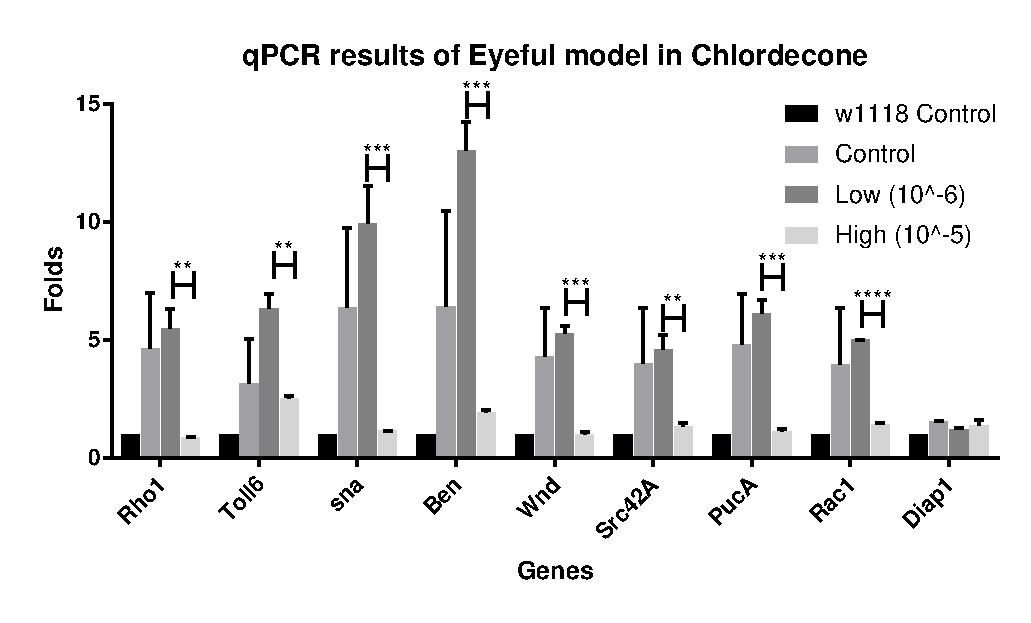
\includegraphics[width=1\textwidth,angle=0]{image/Data4.eps}
    \caption{qPCR results}
    \label{qpcr}
\end{figure}

From the results, we can find that except the Diap1, other 8 genes showed significantly difference (more than ** significance in t test) in mRNA level when treated with different concentration of Chlordecone. However, the transcription level of these genes are not in proportion to the Chlordecone concentration, that is, the relation between Chlordecone concentration and transcription level of these genes is not linear. This indicates a possible hormesis phenomenon of these genes when the fly is treated with POPs like Chlordecone. 

The results of our qPCR is consistent with the result of our previous observation of the tumor metastases in the eyeful model when treated with Chlordecone. Many of the selected genes in our qPCR showed higher transcription in low Chlordecone concentration environment, while in high Chlordecone concentration environment, the transcription level is a little lower, and the tumor metastases ratio of the flies follows the same trend. This may suggest the connection between POPs treatment, suspicious relevant pathways and the phenotype.